%%%%%%%%%%%%%%%%%%%%%%%%%%%%%%%%%%%%%%%%%%%%%%%%%%%%%%%%%%%%%%%%%%%%
%%%%%%%%%%%%%%%%%%%%%%%%%%%%%%%%%%%%%%%%%%%%%%%%%%%%%%%%%%%%%%%%%%%%
\section{Introdução} % Sections can be created in order to organize your presentation into discrete blocks, all sections and subsections are automatically printed in the table of contents as an overview of the talk


%\subsection{Referencial teórico} % A subsection can be created just before a set of slides with a common theme to further break down your presentation into chunks

\begin{frame}
\frametitle{Robótica}
\begin{columns}
	\column{0.35\linewidth}
	\begin{itemize}
	\item Industriais
	\item Médicos
	\item Móveis
		\begin{itemize}
		\item Com pernas (\textit{legged})
		\item Com rodas (\textit{wheeled})
		\end{itemize}
	\end{itemize}

	\column{0.7\linewidth}
	 \begin{figure}[h]
     \centering
     \captionsetup{width=\textwidth,font=footnotesize,textfont=bf}
     \begin{subfigure}[b]{0.5\textwidth}
 	\centering
         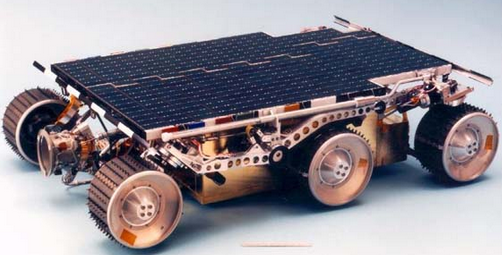
\includegraphics[width=\textwidth,height=\textheight,keepaspectratio]{Figuras/nasa.png}
         \caption{\centering \label{fig:Testen}}
     \end{subfigure}
     
     \begin{subfigure}[b]{0.5\textwidth}
 	\centering
         \includegraphics[width=\textwidth,height=5\textheight,keepaspectratio]{Figuras/Boston.png}
         \caption{\centering \label{fig:Testeo}}
     \end{subfigure}
	\caption{Robôs móveis: (a) Robô Sojourner (NASA,1997);(b) \textit{Legged Squad Support System} (DYNAMICS,2016)}
 \end{figure}
	
\end{columns}
\end{frame}

%------------------------------------------------

\begin{frame}
\frametitle{Controle de tempo contínuo}
\begin{columns}
	\column{0.45\linewidth}
	\begin{itemize}
	\item Malha aberta
	\item Malha fechada
	\item Controlador
		\begin{itemize}
		\item Proporcional
		\item Integral
		\item Derivativa
		\end{itemize}
	\end{itemize}
	
	\column{0.6\linewidth}
	\begin{figure}[h]
     \centering
     \captionsetup{width=\textwidth,font=footnotesize,textfont=bf}
     \begin{subfigure}[b]{\textwidth}
 	\centering
         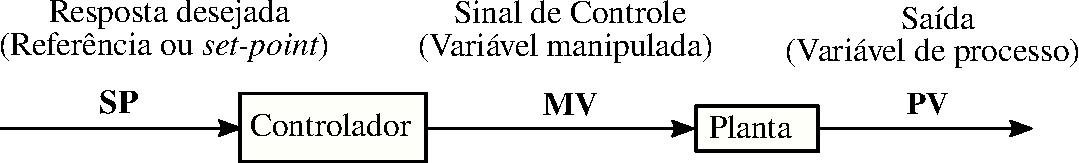
\includegraphics[width=\textwidth,height=\textheight,keepaspectratio]{Figuras/MalhaAberta.pdf}
         \caption{\centering \label{fig:jkl}}
     \end{subfigure}
     
     \begin{subfigure}[b]{\textwidth}
 	\centering
         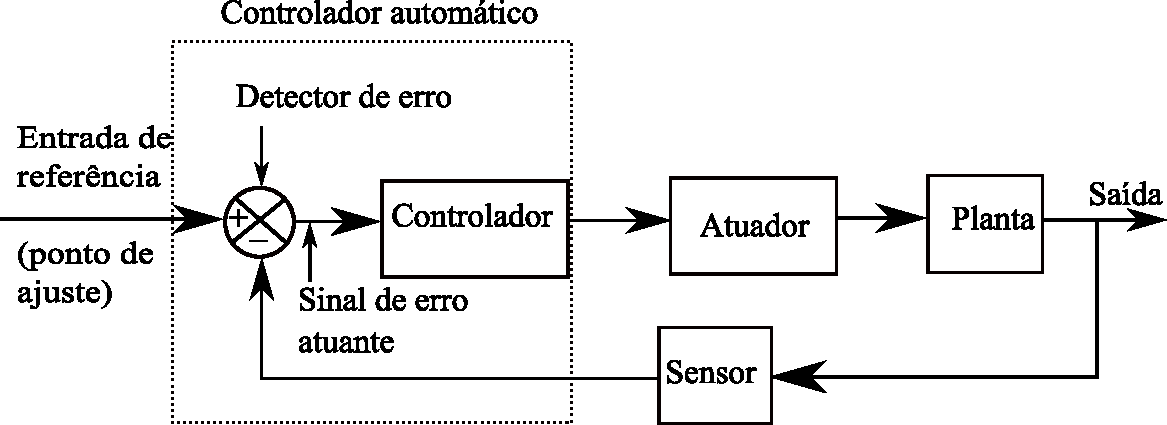
\includegraphics[width=\textwidth,height=5\textheight,keepaspectratio]{Figuras/Controlador.pdf}
         \caption{\centering \label{fig:ppolk}}
     \end{subfigure}
	\caption{Diagramas de controle: (a) Malha aberta;(b) Malha fechada com controlador}
 \end{figure}
	
\end{columns}
\end{frame}

%------------------------------------------------

\begin{frame}
\frametitle{Controle a eventos discretos}
\begin{columns}
	\column{0.3\linewidth}
	\begin{itemize}
	\item Eventos discretos
	\item Autômato
		\begin{itemize}
		\item Moore
		\item Mealy
		\end{itemize}
	\end{itemize}
	
	\column{0.7\linewidth}
	\begin{figure}[h]
     \centering
     \captionsetup{width=0.85\textwidth,font=footnotesize,textfont=bf}
     \begin{subfigure}[b]{\textwidth}
 	\centering
         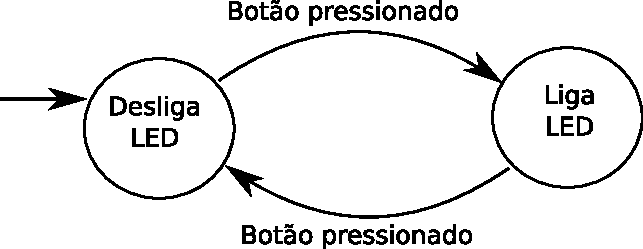
\includegraphics[width=0.85\textwidth,height=\textheight,keepaspectratio]{Figuras/moore.pdf}
         \caption{\centering \label{fig:moore}}
     \end{subfigure}
     
     \begin{subfigure}[b]{\textwidth}
 	\centering
         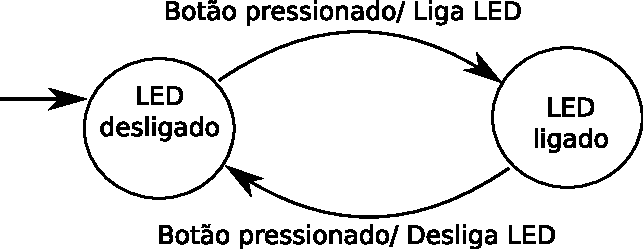
\includegraphics[width=0.85\textwidth,height=5\textheight,keepaspectratio]{Figuras/mealy.pdf}
         \caption{\centering \label{fig:mealy}}
     \end{subfigure}
	\caption{Autômatos: (a) Moore; (b) Mealy (CASSANDRAS;LAFORTUNE;2008,p.43)}
 \end{figure}
	
\end{columns}
\end{frame}


\begin{frame}
\frametitle{Trabalho de Petry (2016)}
\begin{columns}
	\column{0.3\linewidth}
	\begin{itemize}
	\item Controle híbrido
	\item Controlador PID
	\item Lógica \textit{fuzzy}
	\end{itemize}
	
	\column{0.7\linewidth}
	\begin{figure}[h]
     \centering
     \captionsetup{width=0.6\textwidth,font=footnotesize,textfont=bf}
     \begin{subfigure}[b]{0.3\textwidth}
 	\centering
         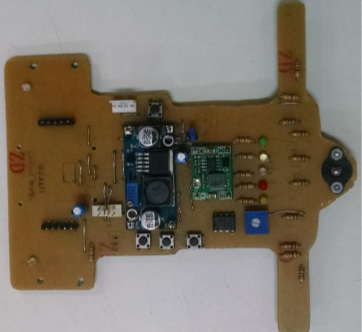
\includegraphics[width=1\textwidth,height=0.4\textheight]{Figuras/marcio1.png}
         \caption{\centering \label{fig:marcio1}}
     \end{subfigure}
	~     
     \begin{subfigure}[b]{0.3\textwidth}
 	\centering
         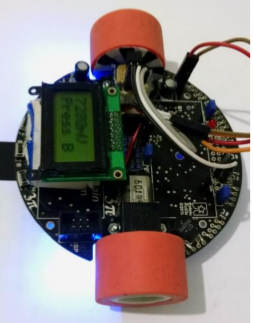
\includegraphics[width=1\textwidth,height=0.4\textheight]{Figuras/polulumod.png}
         \caption{\centering \label{fig:pololumarcio}}
     \end{subfigure}
	\caption{Robôs de Petry (2016): (a) \textit{Alpha project}; (b) Pololu 3pi modificado}
 \end{figure}
	
\end{columns}
\end{frame}

%------------------------------------------------

\begin{frame}
\frametitle{Blocks of Highlighted Text}
\begin{block}{Block 1}
Lorem ipsum dolor sit amet, consectetur adipiscing elit. Integer lectus nisl, ultricies in feugiat rutrum, porttitor sit amet augue. Aliquam ut tortor mauris. Sed volutpat ante purus, quis accumsan dolor.
\end{block}

\begin{block}{Block 2}
Pellentesque sed tellus purus. Class aptent taciti sociosqu ad litora torquent per conubia nostra, per inceptos himenaeos. Vestibulum quis magna at risus dictum tempor eu vitae velit.
\end{block}

\begin{block}{Block 3}
Suspendisse tincidunt sagittis gravida. Curabitur condimentum, enim sed venenatis rutrum, ipsum neque consectetur orci, sed blandit justo nisi ac lacus.
\end{block}
\end{frame}

%------------------------------------------------

\begin{frame}
\frametitle{Multiple Columns}
\begin{columns}[c] % The "c" option specifies centered vertical alignment while the "t" option is used for top vertical alignment

\column{.45\textwidth} % Left column and width
\textbf{Heading}
\begin{enumerate}
\item Statement
\item Explanation
\item Example
\end{enumerate}

\column{.5\textwidth} % Right column and width
Lorem ipsum dolor sit amet, consectetur adipiscing elit. Integer lectus nisl, ultricies in feugiat rutrum, porttitor sit amet augue. Aliquam ut tortor mauris. Sed volutpat ante purus, quis accumsan dolor.

\end{columns}
\end{frame}

%------------------------------------------------
\subsection{Justificativa}



\begin{frame}
\frametitle{Justificativa}

\begin{itemize}
\item ART (\textit{ Autonomous Rail Rapid Transit} ou Trilho Autônomo de Trânsito Rápido)
\item Trem em Zhuzhou (China)
\end{itemize}

\begin{figure}[]
 \centering
 \captionsetup{width=0.65\textwidth,font=footnotesize,textfont=bf}
 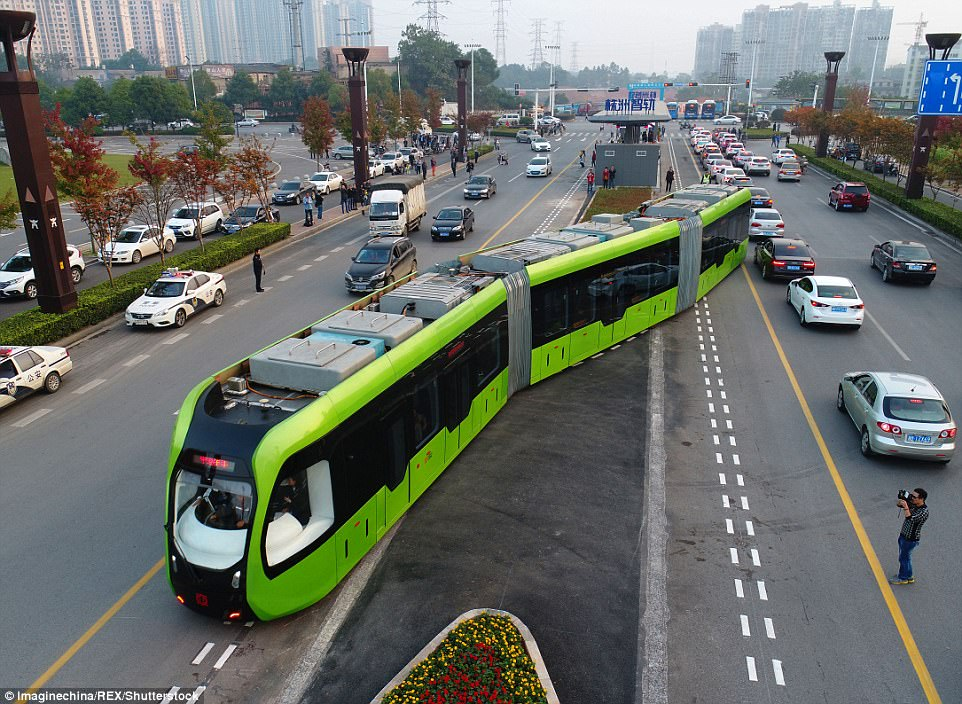
\includegraphics[width=0.65\textwidth,keepaspectratio]{Figuras/Trem.jpg}
 \caption{Trem sobre trilhos virtuais (DAILYMAIL, 2017)}
\end{figure}


\end{frame}


%%%%%%%%%%%%%%%%%%%%%%% EOF %%%%%%%%%%%%%%%%%%%%%%%%%%%%